% Chapter 6: VAR and Granger Causality
% Harvard-quality academic presentation
% Bachelor program, Bucharest University of Economic Studies

\documentclass[9pt, aspectratio=169, t]{beamer}

% Ensure content fits on slides
\setbeamersize{text margin left=8mm, text margin right=8mm}

%=============================================================================
% THEME AND STYLE CONFIGURATION
%=============================================================================
\usetheme{default}
% Using default theme for clean header/footer control

% Color Palette (matching Redispatch PDF)
\definecolor{MainBlue}{RGB}{26, 58, 110}
\definecolor{AccentBlue}{RGB}{26, 58, 110}
\definecolor{IDAred}{RGB}{205, 0, 0}
\definecolor{DarkGray}{RGB}{51, 51, 51}
\definecolor{MediumGray}{RGB}{128, 128, 128}
\definecolor{LightGray}{RGB}{248, 248, 248}
\definecolor{VeryLightGray}{RGB}{235, 235, 235}
\definecolor{KeynoteGray}{RGB}{218, 218, 218}
\definecolor{SectionGray}{RGB}{120, 120, 120}
\definecolor{FooterGray}{RGB}{100, 100, 100}
\definecolor{Crimson}{RGB}{220, 53, 69}
\definecolor{Forest}{RGB}{46, 125, 50}
\definecolor{Amber}{RGB}{181, 133, 63}
\definecolor{Orange}{RGB}{230, 126, 34}
\definecolor{Purple}{RGB}{142, 68, 173}

% Gradient background (exact Keynote 315° gradient: white to RGB 218,218,218)
\setbeamertemplate{background}{%
    \begin{tikzpicture}[remember picture, overlay]
        \shade[shading=axis, shading angle=315,
        top color=white, bottom color=KeynoteGray]
        (current page.south west) rectangle (current page.north east);
    \end{tikzpicture}%
}
% Fallback solid color for compatibility
\setbeamercolor{background canvas}{bg=}

\setbeamercolor{palette primary}{bg=MainBlue, fg=white}
\setbeamercolor{palette secondary}{bg=MainBlue!85, fg=white}
\setbeamercolor{palette tertiary}{bg=MainBlue!70, fg=white}
\setbeamercolor{structure}{fg=MainBlue}
\setbeamercolor{title}{fg=IDAred}
\setbeamercolor{frametitle}{fg=IDAred, bg=}
\setbeamercolor{block title}{bg=MainBlue, fg=white}
\setbeamercolor{block body}{bg=VeryLightGray, fg=DarkGray}
\setbeamercolor{block title alerted}{bg=Crimson, fg=white}
\setbeamercolor{block body alerted}{bg=Crimson!8, fg=DarkGray}
\setbeamercolor{block title example}{bg=Forest, fg=white}
\setbeamercolor{block body example}{bg=Forest!8, fg=DarkGray}
\setbeamercolor{item}{fg=MainBlue}

% Footer colors (override Madrid theme blue)
\setbeamercolor{author in head/foot}{fg=FooterGray, bg=}
\setbeamercolor{title in head/foot}{fg=FooterGray, bg=}
\setbeamercolor{date in head/foot}{fg=FooterGray, bg=}
\setbeamercolor{section in head/foot}{fg=FooterGray, bg=}
\setbeamercolor{subsection in head/foot}{fg=FooterGray, bg=}

% Bullet styles (apply everywhere including blocks)
\setbeamertemplate{itemize item}{\color{MainBlue}$\boxdot$}
\setbeamertemplate{itemize subitem}{\color{MainBlue}$\blacktriangleright$}
\setbeamertemplate{itemize subsubitem}{\color{MainBlue}\tiny$\bullet$}
\setbeamertemplate{itemize/enumerate body begin}{\normalsize}
\setbeamertemplate{itemize/enumerate subbody begin}{\normalsize}

% Item spacing
\setlength{\leftmargini}{1.5em}
\setlength{\leftmarginii}{1.5em}

\setbeamertemplate{navigation symbols}{}

% TOC with bullets
\setbeamertemplate{section in toc}{\color{MainBlue}$\boxdot$\hspace{0.5em}\inserttocsection}

%=============================================================================
% CUSTOM HEADLINE
%=============================================================================
\setbeamertemplate{headline}{%
    \vskip10pt%
    \hbox to \paperwidth{%
        \hskip0.5cm%
        {\small\color{FooterGray}\renewcommand{\hyperlink}[2]{##2}\insertsectionhead}%
        \hfill%
        \textcolor{FooterGray}{\small\insertframenumber}%
        \hskip0.5cm%
    }%
    \vskip4pt%
    {\color{FooterGray}\hrule height 0.4pt}%
}

%=============================================================================
% CUSTOM FOOTER
%=============================================================================
\usepackage{fontawesome5}

\setbeamertemplate{footline}{%
    {\color{FooterGray}\hrule height 0.4pt}%
    \vskip4pt%
    \hbox to \paperwidth{%
        \hskip0.5cm%
        \textcolor{FooterGray}{\small Time Series Analysis and Forecasting}%
        \hfill%
        \raisebox{-0.1em}{%
            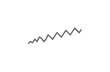
\begin{tikzpicture}[x=0.08em, y=0.08em, line width=0.4pt]
                \draw[FooterGray] (0,3) -- (1,4) -- (2,3.5) -- (3,5) -- (4,4) -- (5,6) -- (6,5.5) -- (7,4) -- (8,5) -- (9,7) -- (10,6) -- (11,5) -- (12,6.5) -- (13,8) -- (14,7) -- (15,6) -- (16,7.5) -- (17,9) -- (18,8) -- (19,7) -- (20,8.5) -- (21,10) -- (22,9) -- (23,8) -- (24,9.5);
            \end{tikzpicture}%
        }%
        \hskip0.5cm%
    }%
    \vskip6pt%
}

%=============================================================================
% PACKAGES
%=============================================================================
\usepackage[utf8]{inputenc}
\usepackage[T1]{fontenc}
\usepackage{amsmath, amssymb, amsthm}
\usepackage{mathtools}
\usepackage{bm}
\usepackage{tikz}
\usetikzlibrary{arrows.meta, positioning, shapes, calc, decorations.pathreplacing, shadings}
\usepackage{booktabs}
\usepackage{multirow}
\usepackage{array}
\usepackage{graphicx}
\usepackage{hyperref}
\usepackage{colortbl}
\hypersetup{colorlinks=true, linkcolor=MainBlue, urlcolor=MainBlue}
\graphicspath{{../logos/}{../charts/}}

%=============================================================================
% QUANTLET COMMAND
%=============================================================================
\newcommand{\quantlet}[2]{%
    \begin{tikzpicture}[remember picture, overlay]
        \node[anchor=south east, inner sep=0pt] at ([xshift=-0.5cm, yshift=0.75cm]current page.south east) {%
            \href{#2}{%
                \raisebox{-0.1em}{\includegraphics[height=0.8em]{ql_logo.png}}%
                \textcolor{MainBlue}{\scriptsize\ #1}%
            }%
        };
    \end{tikzpicture}%
}

%=============================================================================
% CUSTOM TITLE PAGE
%=============================================================================
\defbeamertemplate*{title page}{hybrid}[1][]
{
    \vspace{0.2cm}
    % Logos row - top header (with clickable links)
    \begin{center}
        \href{https://www.ase.ro}{\includegraphics[height=1.0cm]{ase_logo.png}}\hspace{0.3cm}%
        \href{https://theida.net}{\includegraphics[height=1.0cm]{ida_logo.png}}\hspace{0.3cm}%
        \href{https://blockchain-research-center.com}{\includegraphics[height=1.0cm]{brc_logo.png}}\hspace{0.3cm}%
        \href{https://www.ai4efin.ase.ro}{\includegraphics[height=1.0cm]{ai4efin_logo.png}}\hspace{0.3cm}%
        \href{https://ipe.ro/new}{\includegraphics[height=1.0cm]{acad_logo.png}}\hspace{0.3cm}%
        \href{https://www.digital-finance-msca.com}{\includegraphics[height=1.0cm]{msca_logo.png}}%
    \end{center}

    \vspace{0.6cm}

    % Main title with Q logos on sides (with clickable links)
    \begin{center}
        \begin{minipage}{0.1\textwidth}
            \centering
            \href{https://quantlet.com}{\includegraphics[height=1.1cm]{ql_logo.png}}
        \end{minipage}%
        \begin{minipage}{0.78\textwidth}
            \centering
            {\LARGE\bfseries\usebeamercolor[fg]{title}\inserttitle}

            \vspace{0.3cm}

            {\usebeamerfont{subtitle}\usebeamercolor[fg]{title}\insertsubtitle}
        \end{minipage}%
        \begin{minipage}{0.1\textwidth}
            \centering
            \href{https://quantinar.com}{\includegraphics[height=1.1cm]{qr_logo.png}}
        \end{minipage}
    \end{center}

    \vspace{0.6cm}

    % Authors (left aligned)
    \hspace{0.5cm}{\usebeamerfont{author}\insertauthor}

    \vspace{0.3cm}

    % Institute/Affiliations (left aligned)
    \hspace{0.5cm}\begin{minipage}[t]{0.9\textwidth}
        \raggedright\small\insertinstitute
    \end{minipage}
}

%=============================================================================
% THEOREM ENVIRONMENTS
%=============================================================================
\theoremstyle{definition}
\setbeamertemplate{theorems}[numbered]
\newtheorem{defn}{Definition}
\newtheorem{thm}{Theorem}
\newtheorem{prop}{Proposition}
\newtheorem{rmk}{Remark}

%=============================================================================
% CUSTOM COMMANDS
%=============================================================================
\newcommand{\E}{\mathbb{E}}
\newcommand{\Var}{\text{Var}}
\newcommand{\Cov}{\text{Cov}}
\newcommand{\Corr}{\text{Corr}}
\newcommand{\R}{\mathbb{R}}
\newcommand{\N}{\mathbb{N}}
\newcommand{\Z}{\mathbb{Z}}
\newcommand{\B}{\mathbf{B}}
\newcommand{\imark}{\textcolor{MainBlue}{\textbullet}}
\newcommand{\RMSE}{\text{RMSE}}
\newcommand{\MAE}{\text{MAE}}
\newcommand{\MAPE}{\text{MAPE}}
\newcommand{\bA}{\mathbf{A}}
\newcommand{\bSigma}{\boldsymbol{\Sigma}}
\newcommand{\bepsilon}{\boldsymbol{\varepsilon}}
\newcommand{\bY}{\mathbf{Y}}

%=============================================================================
% TITLE INFORMATION
%=============================================================================
\title[Time Series Analysis]{Time Series Analysis and Forecasting}
\subtitle{Chapter 6: VAR and Granger Causality}
\author[D.T. Pele]{Daniel Traian PELE}
\institute{Bucharest University of Economic Studies\\
IDA Institute Digital Assets\\
Blockchain Research Center\\
AI4EFin Artificial Intelligence for Energy Finance\\
Romanian Academy, Institute for Economic Forecasting\\
MSCA Digital Finance}
\date{}

\begin{document}

% Title page (no header/footer)
{
\setbeamertemplate{headline}{}
\setbeamertemplate{footline}{}
\begin{frame}
    \titlepage
\end{frame}
}

%=============================================================================
% TABLE OF CONTENTS
%=============================================================================
\begin{frame}{Outline}
    \tableofcontents
\end{frame}

%=============================================================================
% MOTIVATION
%=============================================================================
\section{Motivation}

\begin{frame}{Motivating Example: Macroeconomic Dynamics}
    \vspace{-0.3cm}
    \begin{center}
        \includegraphics[width=0.88\textwidth, height=0.62\textheight, keepaspectratio]{charts/ch5_motivation_econ.pdf}
    \end{center}
    \vspace{-0.2cm}
    {\footnotesize
    \begin{itemize}
        \item Economic variables are \textbf{interconnected}: GDP affects unemployment, inflation affects interest rates
        \item Changes in one variable \textbf{propagate} through the system
        \item Understanding these dynamics requires \textbf{multivariate} analysis
    \end{itemize}
    }
    \quantlet{TSA\_charts/ch5\_motivation\_econ}{https://github.com/QuantLet/TSA/tree/main/TSA_charts/ch5_motivation_econ}
\end{frame}

\begin{frame}{The Key Insight: Variables Interact}
    \vspace{-0.3cm}
    \begin{center}
        \includegraphics[width=0.85\textwidth, height=0.60\textheight, keepaspectratio]{charts/ch5_motivation_scatter.pdf}
    \end{center}
    \vspace{-0.2cm}
    {\footnotesize
    \begin{itemize}
        \item \textbf{Okun's Law}: Higher GDP growth $\Rightarrow$ lower unemployment
        \item \textbf{Taylor Rule}: Higher inflation $\Rightarrow$ higher interest rates
        \item \textbf{Phillips Curve}: Unemployment-inflation tradeoff
    \end{itemize}
    }
    \quantlet{TSA\_charts/ch5\_motivation\_scatter}{https://github.com/QuantLet/TSA/tree/main/TSA_charts/ch5_motivation_scatter}
\end{frame}

\begin{frame}{Lead-Lag Relationships}
    \vspace{-0.3cm}
    \begin{center}
        \includegraphics[width=0.88\textwidth, height=0.62\textheight, keepaspectratio]{charts/ch5_motivation_leadlag.pdf}
    \end{center}
    \vspace{-0.2cm}
    {\footnotesize
    \begin{itemize}
        \item Some variables \textbf{lead} others: stock market predicts economic activity
        \item Cross-correlation reveals the \textbf{timing} of relationships
        \item Peak correlation at lag 4: stock market leads unemployment by $\sim$4 months
    \end{itemize}
    }
    \quantlet{TSA\_charts/ch5\_motivation\_leadlag}{https://github.com/QuantLet/TSA/tree/main/TSA_charts/ch5_motivation_leadlag}
\end{frame}

\begin{frame}{Why Univariate Models Are Not Enough}
    \vspace{-0.4cm}
    \begin{center}
        \includegraphics[width=0.90\textwidth, height=0.55\textheight, keepaspectratio]{charts/ch5_motivation_univariate.pdf}
    \end{center}
    \vspace{-0.3cm}
    {\footnotesize
    \begin{alertblock}{The Problem}
        ARIMA models each variable \textbf{in isolation}---ignoring valuable information from other variables!
    \end{alertblock}
    \begin{exampleblock}{The Solution}
        \textbf{VAR models} capture the joint dynamics and feedback effects between multiple time series.
    \end{exampleblock}
    }
    \quantlet{TSA\_charts/ch5\_motivation\_univariate}{https://github.com/QuantLet/TSA/tree/main/TSA_charts/ch5_motivation_univariate}
\end{frame}

\begin{frame}{What We'll Learn Today}
    \begin{block}{Core Concepts}
        \begin{enumerate}
            \item \textbf{VAR Models}: How to model multiple time series jointly
            \item \textbf{Granger Causality}: Does $X$ help predict $Y$?
            \item \textbf{Impulse Response Functions}: How do shocks propagate?
            \item \textbf{Variance Decomposition}: What drives each variable?
        \end{enumerate}
    \end{block}

    \vspace{0.2cm}

    \begin{exampleblock}{Applications}
        \begin{itemize}
            \item Macroeconomic policy analysis (monetary policy effects)
            \item Financial market dynamics (stock-bond relationships)
            \item Business cycle analysis (leading indicators)
            \item Risk management (volatility transmission)
        \end{itemize}
    \end{exampleblock}
\end{frame}

%=============================================================================
% SECTION 1: INTRODUCTION
%=============================================================================
\section{Introduction to Multivariate Time Series}

\begin{frame}{Multivariate Time Series Notation}
    \begin{block}{Vector of Variables}
        Let $\bY_t = (Y_{1t}, Y_{2t}, \ldots, Y_{Kt})'$ be a $K \times 1$ vector of time series.

        \vspace{0.2cm}
        Example with $K=2$:
        $$\bY_t = \begin{pmatrix} Y_{1t} \\ Y_{2t} \end{pmatrix} = \begin{pmatrix} \text{GDP growth}_t \\ \text{Inflation}_t \end{pmatrix}$$
    \end{block}

    \vspace{0.15cm}

    \begin{block}{Key Questions}
        \begin{enumerate}
            \item Does $Y_1$ help predict $Y_2$? (Granger causality)
            \item How do shocks to $Y_1$ affect $Y_2$? (Impulse responses)
            \item What proportion of $Y_2$'s variance is due to $Y_1$? (Variance decomposition)
        \end{enumerate}
    \end{block}
\end{frame}

\begin{frame}{Multivariate Stationarity}
    \begin{block}{Definition: Weak Stationarity}
        A $K$-dimensional time series $\bY_t$ is \textbf{weakly stationary} if:
        \begin{enumerate}
            \item $\E[\bY_t] = \boldsymbol{\mu}$ (constant mean vector)
            \item $\Cov(\bY_t, \bY_{t-h}) = \boldsymbol{\Gamma}(h)$ depends only on $h$, not $t$
        \end{enumerate}
    \end{block}

    \vspace{0.15cm}

    \begin{block}{Autocovariance Matrix}
        $$\boldsymbol{\Gamma}(h) = \E[(\bY_t - \boldsymbol{\mu})(\bY_{t-h} - \boldsymbol{\mu})'] = \begin{pmatrix} \gamma_{11}(h) & \gamma_{12}(h) \\ \gamma_{21}(h) & \gamma_{22}(h) \end{pmatrix}$$

        Note: $\boldsymbol{\Gamma}(-h) = \boldsymbol{\Gamma}(h)'$ (transpose, not equal!)
    \end{block}
\end{frame}

\begin{frame}{Cross-Covariance Properties}
    {\small
    \hfill\begin{minipage}{0.9\textwidth}
    \begin{block}{Cross-Covariance Function}
        For variables $Y_{it}$ and $Y_{jt}$:
        $$\gamma_{ij}(h) = \Cov(Y_{it}, Y_{j,t-h}) = \E[(Y_{it} - \mu_i)(Y_{j,t-h} - \mu_j)]$$
    \end{block}

    \begin{alertblock}{Key Difference from Univariate Case}
        \begin{itemize}\setlength{\itemsep}{0pt}
            \item In general: $\gamma_{ij}(h) \neq \gamma_{ij}(-h)$
            \item But: $\gamma_{ij}(h) = \gamma_{ji}(-h)$
            \item The cross-covariance matrix is \textbf{not symmetric} for $h \neq 0$
        \end{itemize}
    \end{alertblock}

    \begin{exampleblock}{Example}
        If $Y_1$ leads $Y_2$: $\gamma_{12}(h) > 0$ for $h > 0$ but $\gamma_{12}(h) \approx 0$ for $h < 0$
    \end{exampleblock}
    \end{minipage}
    }
\end{frame}

\begin{frame}{Correlation Matrix Function}
    \begin{block}{Definition}
        The \textbf{autocorrelation matrix} at lag $h$:
        $$\mathbf{R}(h) = \mathbf{D}^{-1} \boldsymbol{\Gamma}(h) \mathbf{D}^{-1}$$

        where $\mathbf{D} = \text{diag}(\sigma_1, \sigma_2, \ldots, \sigma_K)$ and $\sigma_i = \sqrt{\gamma_{ii}(0)}$
    \end{block}

    \vspace{0.15cm}

    \begin{exampleblock}{For Bivariate Case}
        $$\mathbf{R}(h) = \begin{pmatrix} \rho_{11}(h) & \rho_{12}(h) \\ \rho_{21}(h) & \rho_{22}(h) \end{pmatrix}$$

        where $\rho_{ij}(h) = \frac{\gamma_{ij}(h)}{\sigma_i \sigma_j}$

        \vspace{0.2cm}
        Diagonal elements: usual ACFs; Off-diagonal: cross-correlations
    \end{exampleblock}
\end{frame}

%=============================================================================
% SECTION 2: VAR MODELS
%=============================================================================
\section{Vector Autoregression (VAR)}

\begin{frame}{The VAR(p) Model}
    \begin{block}{Definition}
        A \textbf{VAR(p)} model for $K$ variables:
        $$\bY_t = \mathbf{c} + \bA_1 \bY_{t-1} + \bA_2 \bY_{t-2} + \cdots + \bA_p \bY_{t-p} + \bepsilon_t$$

        where:
        \begin{itemize}
            \item $\bY_t$: $K \times 1$ vector of endogenous variables
            \item $\mathbf{c}$: $K \times 1$ vector of constants
            \item $\bA_i$: $K \times K$ coefficient matrices
            \item $\bepsilon_t$: $K \times 1$ vector of error terms with $\E[\bepsilon_t] = \mathbf{0}$, $\E[\bepsilon_t \bepsilon_t'] = \bSigma$
        \end{itemize}
    \end{block}
\end{frame}

\begin{frame}{VAR(1) with Two Variables}
    \begin{block}{Bivariate VAR(1)}
        $$\begin{pmatrix} Y_{1t} \\ Y_{2t} \end{pmatrix} = \begin{pmatrix} c_1 \\ c_2 \end{pmatrix} + \begin{pmatrix} a_{11} & a_{12} \\ a_{21} & a_{22} \end{pmatrix} \begin{pmatrix} Y_{1,t-1} \\ Y_{2,t-1} \end{pmatrix} + \begin{pmatrix} \varepsilon_{1t} \\ \varepsilon_{2t} \end{pmatrix}$$
    \end{block}

    \vspace{0.15cm}

    \begin{exampleblock}{Equation by Equation}
        \begin{align*}
            Y_{1t} &= c_1 + a_{11} Y_{1,t-1} + a_{12} Y_{2,t-1} + \varepsilon_{1t} \\
            Y_{2t} &= c_2 + a_{21} Y_{1,t-1} + a_{22} Y_{2,t-1} + \varepsilon_{2t}
        \end{align*}

        \textbf{Key insight}: Each equation includes lags of \textbf{all} variables!
    \end{exampleblock}
\end{frame}

\begin{frame}{Numerical Example: VAR(1)}
    {\small
    \hfill\begin{minipage}{0.9\textwidth}
    \begin{exampleblock}{Specific VAR(1) Model}
        $$\begin{pmatrix} Y_{1t} \\ Y_{2t} \end{pmatrix} = \begin{pmatrix} 0.5 \\ 0.3 \end{pmatrix} + \begin{pmatrix} 0.7 & 0.2 \\ -0.1 & 0.6 \end{pmatrix} \begin{pmatrix} Y_{1,t-1} \\ Y_{2,t-1} \end{pmatrix} + \begin{pmatrix} \varepsilon_{1t} \\ \varepsilon_{2t} \end{pmatrix}$$
    \end{exampleblock}

    \begin{block}{Interpretation of Coefficients}
        \begin{itemize}\setlength{\itemsep}{0pt}
            \item $a_{11} = 0.7$: A 1-unit increase in $Y_1$ at $t-1$ increases $Y_1$ at $t$ by 0.7
            \item $a_{12} = 0.2$: A 1-unit increase in $Y_2$ at $t-1$ increases $Y_1$ at $t$ by 0.2
            \item $a_{21} = -0.1$: A 1-unit increase in $Y_1$ at $t-1$ \textbf{decreases} $Y_2$ at $t$ by 0.1
            \item $a_{22} = 0.6$:
                \begin{itemize}
                    \item A 1-unit increase in $Y_2$ at $t-1$ increases $Y_2$ at $t$ by 0.6
                \end{itemize}
            \end{itemize}
    \end{block}
    \end{minipage}
    }
\end{frame}

\begin{frame}{VAR(2): Higher Order Dynamics}
    \begin{block}{VAR(2) Specification}
        $\bY_t = \mathbf{c} + \bA_1 \bY_{t-1} + \bA_2 \bY_{t-2} + \bepsilon_t$. For $K=2$: $2 + 2 \times 4 + 2 \times 4 = 18$ parameters!
    \end{block}

    \vspace{0.1cm}

    {\small
    \begin{exampleblock}{Written Out}
        \begin{align*}
            Y_{1t} &= c_1 + a_{11}^{(1)} Y_{1,t-1} + a_{12}^{(1)} Y_{2,t-1} + a_{11}^{(2)} Y_{1,t-2} + a_{12}^{(2)} Y_{2,t-2} + \varepsilon_{1t} \\
            Y_{2t} &= c_2 + a_{21}^{(1)} Y_{1,t-1} + a_{22}^{(1)} Y_{2,t-1} + a_{21}^{(2)} Y_{1,t-2} + a_{22}^{(2)} Y_{2,t-2} + \varepsilon_{2t}
        \end{align*}
    \end{exampleblock}
    }

    \vspace{0.1cm}

    {\footnotesize
    \begin{alertblock}{Curse of Dimensionality}
        VAR($p$) with $K$ variables has $K + pK^2$ parameters. With $K=5$, $p=4$: $5 + 4 \times 25 = 105$ parameters!
    \end{alertblock}
    }
\end{frame}

\begin{frame}{The Companion Form}
    \begin{block}{Converting VAR(p) to VAR(1)}
        Any VAR($p$) can be written as a VAR(1) in \textbf{companion form}:
        $\boldsymbol{\xi}_t = \mathbf{A} \boldsymbol{\xi}_{t-1} + \mathbf{v}_t$
    \end{block}

    \vspace{0.1cm}

    {\small
    \begin{exampleblock}{For VAR(2)}
        $$\underbrace{\begin{pmatrix} \bY_t \\ \bY_{t-1} \end{pmatrix}}_{\boldsymbol{\xi}_t} = \underbrace{\begin{pmatrix} \bA_1 & \bA_2 \\ \mathbf{I}_K & \mathbf{0} \end{pmatrix}}_{\mathbf{A}} \underbrace{\begin{pmatrix} \bY_{t-1} \\ \bY_{t-2} \end{pmatrix}}_{\boldsymbol{\xi}_{t-1}} + \underbrace{\begin{pmatrix} \bepsilon_t \\ \mathbf{0} \end{pmatrix}}_{\mathbf{v}_t}$$
    \end{exampleblock}
    }

    \vspace{0.1cm}

    {\footnotesize
    \begin{block}{Why Useful?}
        Stationarity, forecasting, and IRFs are easier in companion form. Matrix $\mathbf{A}$ is $Kp \times Kp$.
    \end{block}
    }
\end{frame}

\begin{frame}{VAR Process: GDP and Unemployment (FRED)}
    \vspace{-0.3cm}
    \begin{center}
        \includegraphics[width=0.82\textwidth, height=0.58\textheight, keepaspectratio]{charts/ch5_var_simulation.pdf}
    \end{center}
    \vspace{-0.2cm}
    {\footnotesize
    \begin{itemize}
        \item \textbf{Data}: US GDP Growth (GDPC1) and Unemployment Rate (UNRATE) from FRED
        \item Each variable responds to both its own past and the other variable's past
        \item Classic example of macroeconomic interdependence (Okun's Law)
    \end{itemize}
    }
    \quantlet{TSA\_charts/ch5\_var\_simulation}{https://github.com/QuantLet/TSA/tree/main/TSA_charts/ch5_var_simulation}
\end{frame}

\begin{frame}{Stationarity of VAR}
    \begin{block}{Stability Condition}
        VAR(p) is \textbf{stable} (stationary) if all roots of:
        $$\det(\mathbf{I}_K - \bA_1 z - \bA_2 z^2 - \cdots - \bA_p z^p) = 0$$
        lie \textbf{outside} the unit circle (i.e., $|z| > 1$).
    \end{block}

    \vspace{0.15cm}

    \begin{alertblock}{For VAR(1)}
        The model is stable if all \textbf{eigenvalues} of $\bA_1$ are less than 1 in absolute value.

        \vspace{0.2cm}
        Example: For $\bA_1 = \begin{pmatrix} 0.5 & 0.1 \\ 0.2 & 0.3 \end{pmatrix}$, eigenvalues are $\lambda_1 = 0.6$ and $\lambda_2 = 0.2$.

        Both $< 1$ $\Rightarrow$ stable!
    \end{alertblock}
\end{frame}

\begin{frame}{Computing Eigenvalues: Example}
    {\small
    \hfill\begin{minipage}{0.9\textwidth}
    \begin{block}{For $\bA = \begin{pmatrix} 0.7 & 0.2 \\ -0.1 & 0.6 \end{pmatrix}$}
        Characteristic polynomial: $\det(\bA - \lambda \mathbf{I}) = 0$
        $$\det\begin{pmatrix} 0.7 - \lambda & 0.2 \\ -0.1 & 0.6 - \lambda \end{pmatrix} = (0.7-\lambda)(0.6-\lambda) + 0.02 = 0$$
        $$\lambda^2 - 1.3\lambda + 0.44 = 0$$
    \end{block}

    \begin{exampleblock}{Solution}
        Using quadratic formula:
        $$\lambda = \frac{1.3 \pm \sqrt{1.69 - 1.76}}{2} = \frac{1.3 \pm \sqrt{-0.07}}{2} = 0.65 \pm 0.132i$$

        $|\lambda| = \sqrt{0.65^2 + 0.132^2} = \sqrt{0.44} = 0.663 < 1$ \quad $\checkmark$ Stable!
    \end{exampleblock}
    \end{minipage}
    }
\end{frame}

\begin{frame}{Stability Condition: Visual Interpretation}
    \vspace{-0.3cm}
    \begin{center}
        \includegraphics[width=0.82\textwidth, height=0.58\textheight, keepaspectratio]{charts/ch5_stability_roots.pdf}
    \end{center}
    \vspace{-0.2cm}
    {\footnotesize
    \begin{itemize}
        \item Eigenvalues of the companion matrix must lie inside the unit circle
        \item Complex eigenvalues come in conjugate pairs
        \item If any eigenvalue is outside the circle, the VAR is explosive (non-stationary)
    \end{itemize}
    }
    \quantlet{TSA\_charts/ch5\_stability\_roots}{https://github.com/QuantLet/TSA/tree/main/TSA_charts/ch5_stability_roots}
\end{frame}

\begin{frame}{Mean of a Stationary VAR}
    {\small
    \begin{block}{Unconditional Mean}
        For stationary VAR(1): $\bY_t = \mathbf{c} + \bA \bY_{t-1} + \bepsilon_t$. Since $\E[\bY_t] = \E[\bY_{t-1}] = \boldsymbol{\mu}$:
        $$\boldsymbol{\mu} = \mathbf{c} + \bA \boldsymbol{\mu} \quad \Rightarrow \quad \boldsymbol{\mu} = (\mathbf{I}_K - \bA)^{-1} \mathbf{c}$$
    \end{block}

    \begin{exampleblock}{Example}
        If $\mathbf{c} = \begin{pmatrix} 0.5 \\ 0.3 \end{pmatrix}$ and $\bA = \begin{pmatrix} 0.7 & 0.2 \\ -0.1 & 0.6 \end{pmatrix}$:
        $\boldsymbol{\mu} = \begin{pmatrix} 0.3 & -0.2 \\ 0.1 & 0.4 \end{pmatrix}^{-1} \begin{pmatrix} 0.5 \\ 0.3 \end{pmatrix} = \begin{pmatrix} 2.3 \\ 1.0 \end{pmatrix}$
    \end{exampleblock}
    }
\end{frame}

\begin{frame}{Covariance Structure of VAR(1)}
    {\small
    \hfill\begin{minipage}{0.9\textwidth}
    \begin{block}{Variance-Covariance Matrix $\boldsymbol{\Gamma}(0)$}
        For VAR(1), the variance satisfies the \textbf{discrete Lyapunov equation}:
        $$\boldsymbol{\Gamma}(0) = \bA \boldsymbol{\Gamma}(0) \bA' + \bSigma$$
    \end{block}

    \begin{block}{Autocovariance at Lag $h$}
        $$\boldsymbol{\Gamma}(h) = \bA^h \boldsymbol{\Gamma}(0), \quad h \geq 0$$

        This shows that autocovariances decay geometrically with the eigenvalues of $\bA$.
    \end{block}

    \begin{alertblock}{Solving the Lyapunov Equation}
        Can solve by vectorization:
        $$\text{vec}(\boldsymbol{\Gamma}(0)) = (\mathbf{I}_{K^2} - \bA \otimes \bA)^{-1} \text{vec}(\bSigma)$$
        where $\otimes$ denotes the Kronecker product.
    \end{alertblock}
    \end{minipage}
    }
\end{frame}

\begin{frame}{Estimation of VAR}
    \begin{block}{OLS Estimation}
        Each equation can be estimated by \textbf{OLS separately}:
        $$\hat{\bA} = \left(\sum_{t=1}^{T} \bY_{t-1} \bY_{t-1}'\right)^{-1} \left(\sum_{t=1}^{T} \bY_{t-1} \bY_t'\right)$$

        \vspace{0.2cm}
        This is efficient because all equations have the \textbf{same regressors}.
    \end{block}

    \vspace{0.15cm}

    \begin{block}{Covariance Matrix}
        $$\hat{\bSigma} = \frac{1}{T-Kp-1} \sum_{t=1}^{T} \hat{\bepsilon}_t \hat{\bepsilon}_t'$$

        The errors $\varepsilon_{1t}$ and $\varepsilon_{2t}$ may be \textbf{contemporaneously correlated}.
    \end{block}
\end{frame}

\begin{frame}{Lag Order Selection}
    \begin{block}{Information Criteria}
        Choose $p$ that minimizes:
        \begin{align*}
            \text{AIC}(p) &= \ln|\hat{\bSigma}_p| + \frac{2pK^2}{T} \quad
            \text{BIC}(p) = \ln|\hat{\bSigma}_p| + \frac{pK^2 \ln T}{T}
        \end{align*}
    \end{block}

    \vspace{0.1cm}

    {\footnotesize
    \begin{block}{Guidelines}
        \begin{itemize}\setlength{\itemsep}{0pt}
            \item AIC: larger models (better forecasting); BIC: smaller models (consistent)
            \item Start with $p_{max}$ based on frequency (4 quarterly, 12 monthly)
        \end{itemize}
    \end{block}
    }
\end{frame}

\begin{frame}{Lag Selection: Example}
    \vspace{-0.3cm}
    \begin{center}
        \includegraphics[width=0.82\textwidth, height=0.58\textheight, keepaspectratio]{charts/ch5_lag_selection.pdf}
    \end{center}
    \vspace{-0.2cm}
    {\footnotesize
    \begin{itemize}
        \item Information criteria values for different lag orders
        \item AIC and BIC may suggest different optimal lags
        \item Lower values indicate better model fit (penalized by complexity)
    \end{itemize}
    }
    \quantlet{TSA\_charts/ch5\_lag\_selection}{https://github.com/QuantLet/TSA/tree/main/TSA_charts/ch5_lag_selection}
\end{frame}

\begin{frame}{Restricted VAR Models}
    {\small
    \hfill\begin{minipage}{0.9\textwidth}
    \begin{block}{Why Restrict?}
        Full VAR models can be \textbf{overparameterized}:
        \begin{itemize}\setlength{\itemsep}{0pt}
            \item Many coefficients may be insignificant
            \item Poor forecasting performance
            \item Loss of degrees of freedom
        \end{itemize}
    \end{block}

    \begin{block}{Common Restrictions}
        \begin{itemize}\setlength{\itemsep}{0pt}
            \item \textbf{Zero restrictions}: Set small coefficients to zero
            \item \textbf{Block exogeneity}: Some variables don't affect others
            \item \textbf{Lag exclusion}: Exclude certain lags
        \end{itemize}
    \end{block}

    \begin{alertblock}{Testing Restrictions}
        Use likelihood ratio test:
        $LR = T(\ln|\hat{\bSigma}_R| - \ln|\hat{\bSigma}_U|) \sim \chi^2_r$

        where $r$ = number of restrictions
    \end{alertblock}
    \end{minipage}
    }
\end{frame}

%=============================================================================
% SECTION 3: GRANGER CAUSALITY
%=============================================================================
\section{Granger Causality}

\begin{frame}{What is Granger Causality?}
    \begin{block}{Clive Granger (1969, Nobel Prize 2003)}
        ``$X$ \textbf{Granger-causes} $Y$'' if past values of $X$ help predict $Y$, \textbf{beyond} what past values of $Y$ alone can predict.
    \end{block}

    \vspace{0.15cm}

    \begin{alertblock}{Important Distinction}
        \textbf{Granger causality $\neq$ True causality}

        \begin{itemize}
            \item Granger causality is about \textbf{predictive content}
            \item Does NOT imply economic/structural causation
            \item ``$X$ Granger-causes $Y$'' means:
                \begin{itemize}
                    \item $X$ contains useful information for forecasting $Y$
                \end{itemize}
            \end{itemize}
    \end{alertblock}
\end{frame}

\begin{frame}{Formal Definition}
    \begin{block}{Granger Causality}
        $X$ \textbf{does not Granger-cause} $Y$ if:
        $$\E[Y_t | Y_{t-1}, Y_{t-2}, \ldots, X_{t-1}, X_{t-2}, \ldots] = \E[Y_t | Y_{t-1}, Y_{t-2}, \ldots]$$

        In other words: adding $X$'s history does not improve the prediction of $Y$.
    \end{block}

    \vspace{0.15cm}

    \begin{exampleblock}{In the VAR Context}
        For VAR(1): $Y_{1t} = c_1 + a_{11} Y_{1,t-1} + a_{12} Y_{2,t-1} + \varepsilon_{1t}$

        \vspace{0.2cm}
        $Y_2$ does \textbf{not} Granger-cause $Y_1$ if $a_{12} = 0$.

        \vspace{0.2cm}
        For VAR(p): $Y_2$ does not Granger-cause $Y_1$ if $a_{12}^{(1)} = a_{12}^{(2)} = \cdots = a_{12}^{(p)} = 0$.
    \end{exampleblock}
\end{frame}

\begin{frame}{Testing for Granger Causality}
    \begin{block}{Hypothesis Test}
        \textbf{$H_0$}: $Y_2$ does \textbf{not} Granger-cause $Y_1$

        $$H_0: a_{12}^{(1)} = a_{12}^{(2)} = \cdots = a_{12}^{(p)} = 0$$

        \textbf{$H_1$}: At least one $a_{12}^{(i)} \neq 0$ (Granger causality exists)
    \end{block}

    \vspace{0.15cm}

    \begin{block}{Test Statistic: Wald Test}
        $$F = \frac{(RSS_R - RSS_U)/p}{RSS_U/(T-2p-1)} \sim F_{p, T-2p-1}$$

        where:
        \begin{itemize}
            \item $RSS_R$: Residual sum of squares from restricted model (without $Y_2$ lags)
            \item $RSS_U$: Residual sum of squares from unrestricted model (full VAR)
        \end{itemize}
    \end{block}
\end{frame}

\begin{frame}{Types of Granger Causality}
    \vspace{-0.2cm}
    \begin{center}
    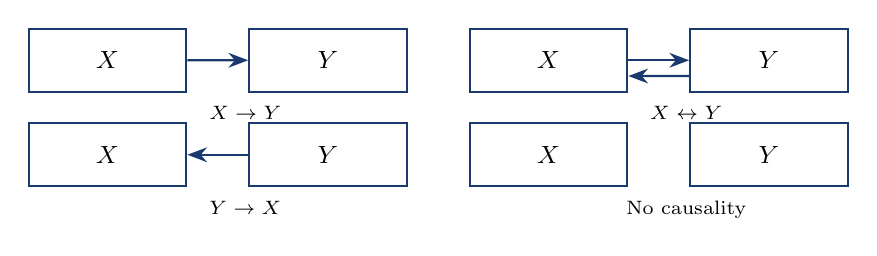
\begin{tikzpicture}[scale=0.8,
        box/.style={rectangle, draw=MainBlue, thick, minimum width=2cm, minimum height=0.8cm, font=\small},
        arrow/.style={-{Stealth[length=2.5mm]}, thick, MainBlue}
    ]
        % Unidirectional X -> Y
        \node[box] (x1) at (0, 1.5) {$X$};
        \node[box] (y1) at (3.5, 1.5) {$Y$};
        \draw[arrow] (x1) -- (y1);
        \node[below=0.05cm of x1, xshift=1.75cm, font=\scriptsize] {$X \rightarrow Y$};

        % Unidirectional Y -> X
        \node[box] (x2) at (0, 0) {$X$};
        \node[box] (y2) at (3.5, 0) {$Y$};
        \draw[arrow] (y2) -- (x2);
        \node[below=0.05cm of x2, xshift=1.75cm, font=\scriptsize] {$Y \rightarrow X$};

        % Bidirectional
        \node[box] (x3) at (7, 1.5) {$X$};
        \node[box] (y3) at (10.5, 1.5) {$Y$};
        \draw[arrow] (x3.east) -- (y3.west);
        \draw[arrow] (y3.west) ++(0, -0.25) -- (x3.east |- {0, 1.25});
        \node[below=0.05cm of x3, xshift=1.75cm, font=\scriptsize] {$X \leftrightarrow Y$};

        % No causality
        \node[box] (x4) at (7, 0) {$X$};
        \node[box] (y4) at (10.5, 0) {$Y$};
        \node[below=0.05cm of x4, xshift=1.75cm, font=\scriptsize] {No causality};
    \end{tikzpicture}
    \end{center}

    \vspace{0.1cm}

    {\footnotesize
    \begin{block}{Economic Examples}
        \begin{itemize}\setlength{\itemsep}{0pt}
            \item Money $\rightarrow$ Output? (monetarist); Stock prices $\leftrightarrow$ Volume (bidirectional)
        \end{itemize}
    \end{block}
    }
\end{frame}

\begin{frame}{Cross-Correlation Function}
    {\small
    \hfill\begin{minipage}{0.9\textwidth}
    \begin{defn}[Cross-Correlation Function]
        The \textbf{cross-correlation} between $X_t$ and $Y_t$ at lag $k$ is:
        $$\rho_{XY}(k) = \frac{\gamma_{XY}(k)}{\sigma_X \sigma_Y} = \frac{\Cov(X_t, Y_{t+k})}{\sqrt{\Var(X_t)\Var(Y_t)}}$$
    \end{defn}

    \begin{block}{Interpretation}
        \begin{itemize}\setlength{\itemsep}{0pt}
            \item $\rho_{XY}(k) > 0$ at $k > 0$: $X$ is positively correlated with future $Y$ (X may lead Y)
            \item $\rho_{XY}(k) > 0$ at $k < 0$: $X$ is positively correlated with past $Y$ (Y may lead X)
        \end{itemize}
    \end{block}

    \begin{alertblock}{Note}
        Unlike ACF, cross-correlation is \textbf{not symmetric}: $\rho_{XY}(k) \neq \rho_{XY}(-k)$ in general.
    \end{alertblock}
    \end{minipage}
    }
\end{frame}

\begin{frame}{Cross-Correlation: Visual Illustration}
    \begin{center}
        \includegraphics[width=0.95\textwidth]{charts/ch5_def_ccf.pdf}
    \end{center}
    \vspace{-0.2cm}
    \small Left: two related series. Right: CCF reveals that $X$ leads $Y$ (significant correlations at positive lags).
    \quantlet{TSA\_charts/ch5\_def\_ccf}{https://github.com/QuantLet/TSA/tree/main/TSA_charts/ch5_def_ccf}
\end{frame}

\begin{frame}{Granger Causality: Practical Considerations}
    \begin{alertblock}{Common Pitfalls}
        \begin{enumerate}
            \item \textbf{Omitted variables}: A third variable $Z$ may cause both $X$ and $Y$
            \item \textbf{Non-stationarity}: Test requires stationary data (or cointegration)
            \item \textbf{Lag selection}: Results can be sensitive to $p$
            \item \textbf{Sample size}: Need sufficient observations
        \end{enumerate}
    \end{alertblock}

    \vspace{0.15cm}

    \begin{block}{Best Practices}
        \begin{itemize}
            \item Test for unit roots first
            \item Use multiple lag selection criteria
            \item Check robustness to different lag lengths
            \item Report results for both directions
        \end{itemize}
    \end{block}
\end{frame}

\begin{frame}{Granger Causality Test: Numerical Example}
    {\small
    \hfill\begin{minipage}{0.9\textwidth}
    \begin{exampleblock}{Testing: Does Money Growth Granger-cause Output?}
        \textbf{Unrestricted model} (VAR with 2 lags):
        $$\Delta Y_t = c + \alpha_1 \Delta Y_{t-1} + \alpha_2 \Delta Y_{t-2} + \beta_1 \Delta M_{t-1} + \beta_2 \Delta M_{t-2} + \varepsilon_t$$

        \textbf{Restricted model} ($H_0$: $\beta_1 = \beta_2 = 0$):
        $$\Delta Y_t = c + \alpha_1 \Delta Y_{t-1} + \alpha_2 \Delta Y_{t-2} + \varepsilon_t$$
    \end{exampleblock}

    \begin{block}{Test Computation}
        With $T = 100$, $RSS_U = 45.2$, $RSS_R = 52.8$:
        $$F = \frac{(52.8 - 45.2)/2}{45.2/(100 - 5)} = \frac{3.8}{0.476} = 7.98$$

        $F_{0.05}(2, 95) = 3.09$ $\Rightarrow$ \textbf{Reject $H_0$}: Money Granger-causes output!
    \end{block}
    \end{minipage}
    }
\end{frame}

\begin{frame}{The Toda-Yamamoto Procedure}
    {\small
    \hfill\begin{minipage}{0.9\textwidth}
    \begin{alertblock}{Problem with Non-Stationary Data}
        Standard Granger test has \textbf{non-standard distributions} when:
        \begin{itemize}\setlength{\itemsep}{0pt}
            \item Variables have unit roots
            \item Variables are cointegrated
        \end{itemize}
    \end{alertblock}

    \begin{block}{Toda-Yamamoto Solution (1995)}
        \begin{enumerate}\setlength{\itemsep}{0pt}
            \item Determine maximum order of integration $d_{max}$
            \item Estimate VAR($p + d_{max}$) in \textbf{levels}
            \item Test restrictions on first $p$ lags only
            \item Extra $d_{max}$ lags are \textbf{not} tested (just for correct distribution)
        \end{enumerate}
    \end{block}

    \begin{exampleblock}{Advantage}
        Wald test has asymptotic $\chi^2$ distribution regardless of cointegration!
    \end{exampleblock}
    \end{minipage}
    }
\end{frame}

\begin{frame}{Instantaneous Causality}
    \begin{block}{Definition}
        $X$ \textbf{instantaneously causes} $Y$ if $\E[Y_t | \Omega_{t-1}, X_t] \neq \E[Y_t | \Omega_{t-1}]$, where $\Omega_{t-1}$ contains all past information.
    \end{block}

    \vspace{0.1cm}

    \begin{block}{Testing in VAR}
        Test whether $\sigma_{12} \neq 0$ in the covariance matrix:
        $\bSigma = \begin{pmatrix} \sigma_1^2 & \sigma_{12} \\ \sigma_{12} & \sigma_2^2 \end{pmatrix}$.
        If $\sigma_{12} = 0$: no instantaneous causality.
    \end{block}

    \vspace{0.1cm}

    {\footnotesize
    \begin{alertblock}{Interpretation}
        Instantaneous causality often reflects \textbf{common shocks} or \textbf{data aggregation}, not true contemporaneous effects.
    \end{alertblock}
    }
\end{frame}

\begin{frame}{Granger Causality in Multiple Systems}
    \begin{block}{Block Exogeneity Test}
        In a VAR with $K > 2$ variables, test whether a \textbf{group} of variables Granger-causes another group.

        \vspace{0.2cm}
        Example: Do financial variables (interest rates, stock prices) Granger-cause real variables (GDP, unemployment)?
    \end{block}

    \vspace{0.15cm}

    \begin{exampleblock}{Test Statistic}
        $$\chi^2 = T \cdot K_1 \cdot p \cdot \left(\ln|\hat{\bSigma}_R| - \ln|\hat{\bSigma}_U|\right) \sim \chi^2_{K_1 \cdot K_2 \cdot p}$$

        where $K_1$ = number of ``caused'' variables, $K_2$ = number of ``causing'' variables
    \end{exampleblock}
\end{frame}

%=============================================================================
% SECTION 4: IMPULSE RESPONSE FUNCTIONS
%=============================================================================
\section{Impulse Response Functions}

\begin{frame}{What are Impulse Response Functions?}
    \begin{block}{Definition}
        An \textbf{Impulse Response Function (IRF)} traces the effect of a one-time shock to one variable on the current and future values of all variables.
    \end{block}

    \vspace{0.15cm}

    \begin{exampleblock}{Question IRFs Answer}
        ``If there is an unexpected 1-unit shock to $Y_1$ today, what happens to $Y_1$ and $Y_2$ over the next $h$ periods?''
    \end{exampleblock}

    \vspace{0.15cm}

    \begin{block}{MA($\infty$) Representation}
        A stable VAR(p) can be written as:
        $$\bY_t = \boldsymbol{\mu} + \sum_{i=0}^{\infty} \boldsymbol{\Phi}_i \bepsilon_{t-i}$$

        The matrices $\boldsymbol{\Phi}_i$ are the \textbf{impulse responses} at horizon $i$.
    \end{block}
\end{frame}

\begin{frame}{Computing IRFs for VAR(1)}
    \begin{block}{For VAR(1): $\bY_t = \mathbf{c} + \bA \bY_{t-1} + \bepsilon_t$}
        The impulse response matrices are:
        $$\boldsymbol{\Phi}_0 = \mathbf{I}_K, \quad \boldsymbol{\Phi}_1 = \bA, \quad \boldsymbol{\Phi}_2 = \bA^2, \quad \ldots, \quad \boldsymbol{\Phi}_h = \bA^h$$
    \end{block}

    \vspace{0.15cm}

    \begin{exampleblock}{Interpretation}
        $[\boldsymbol{\Phi}_h]_{ij}$ = Effect on $Y_i$ at time $t+h$ of a unit shock to $Y_j$ at time $t$

        \vspace{0.2cm}
        For stable VAR: $\boldsymbol{\Phi}_h \rightarrow \mathbf{0}$ as $h \rightarrow \infty$ (shocks die out)
    \end{exampleblock}
\end{frame}

\begin{frame}{Computing IRFs for General VAR(p)}
    {\small
    \hfill\begin{minipage}{0.9\textwidth}
    \begin{block}{Recursive Formula for VAR(p)}
        For $\bY_t = \mathbf{c} + \bA_1\bY_{t-1} + \bA_2\bY_{t-2} + \cdots + \bA_p\bY_{t-p} + \bepsilon_t$:
        $$\boldsymbol{\Phi}_h = \sum_{j=1}^{\min(h,p)} \bA_j \boldsymbol{\Phi}_{h-j}, \quad h = 1, 2, 3, \ldots$$
        with $\boldsymbol{\Phi}_0 = \mathbf{I}_K$ and $\boldsymbol{\Phi}_h = \mathbf{0}$ for $h < 0$.
    \end{block}

    \begin{exampleblock}{Example: VAR(2) IRFs}
        \begin{itemize}\setlength{\itemsep}{0pt}
            \item $\boldsymbol{\Phi}_0 = \mathbf{I}_K$
            \item $\boldsymbol{\Phi}_1 = \bA_1 \boldsymbol{\Phi}_0 = \bA_1$
            \item $\boldsymbol{\Phi}_2 = \bA_1 \boldsymbol{\Phi}_1 + \bA_2 \boldsymbol{\Phi}_0 = \bA_1^2 + \bA_2$
            \item $\boldsymbol{\Phi}_3 = \bA_1 \boldsymbol{\Phi}_2 + \bA_2 \boldsymbol{\Phi}_1 = \bA_1(\bA_1^2 + \bA_2) + \bA_2\bA_1$
        \end{itemize}
    \end{exampleblock}
    \end{minipage}
    }
\end{frame}

\begin{frame}{Orthogonalized IRFs}
    \begin{alertblock}{Problem: Correlated Errors}
        If $\bSigma$ is not diagonal, shocks $\varepsilon_{1t}$ and $\varepsilon_{2t}$ are correlated.

        A shock to ``$Y_1$'' also involves a shock to ``$Y_2$''.
    \end{alertblock}

    \vspace{0.15cm}

    \begin{block}{Solution: Cholesky Decomposition}
        Factor $\bSigma = \mathbf{P}\mathbf{P}'$ where $\mathbf{P}$ is lower triangular.

        Define orthogonalized shocks: $\mathbf{u}_t = \mathbf{P}^{-1}\bepsilon_t$ with $\E[\mathbf{u}_t \mathbf{u}_t'] = \mathbf{I}$

        \vspace{0.2cm}
        Orthogonalized IRFs: $\boldsymbol{\Theta}_h = \boldsymbol{\Phi}_h \mathbf{P}$
    \end{block}

    \vspace{0.2cm}

    {\small
    \begin{alertblock}{Ordering Matters!}
        Cholesky assumes variables ordered from ``most exogenous'' to ``most endogenous''. Results depend on this ordering.
    \end{alertblock}
    }
\end{frame}

\begin{frame}{Impulse Response Functions: Example}
    \vspace{-0.3cm}
    \begin{center}
        \includegraphics[width=0.82\textwidth, height=0.58\textheight, keepaspectratio]{charts/ch5_irf.pdf}
    \end{center}
    \vspace{-0.2cm}
    {\footnotesize
    \begin{itemize}
        \item IRFs show how each variable responds to a one-unit shock over time
        \item Shaded regions represent confidence intervals (uncertainty in estimates)
        \item For stable VAR models, responses converge to zero as the horizon increases
    \end{itemize}
    }
    \quantlet{TSA\_charts/ch5\_irf}{https://github.com/QuantLet/TSA/tree/main/TSA_charts/ch5_irf}
\end{frame}

\begin{frame}{IRF Numerical Example}
    {\small
    \hfill\begin{minipage}{0.9\textwidth}
    \begin{block}{For $\bA = \begin{pmatrix} 0.7 & 0.2 \\ -0.1 & 0.6 \end{pmatrix}$}
        \begin{align*}
            \boldsymbol{\Phi}_0 &= \begin{pmatrix} 1 & 0 \\ 0 & 1 \end{pmatrix} \\
            \boldsymbol{\Phi}_1 &= \bA = \begin{pmatrix} 0.7 & 0.2 \\ -0.1 & 0.6 \end{pmatrix} \\
            \boldsymbol{\Phi}_2 &= \bA^2 = \begin{pmatrix} 0.47 & 0.26 \\ -0.13 & 0.34 \end{pmatrix}
        \end{align*}
    \end{block}

    \begin{exampleblock}{Interpretation}
        \begin{itemize}\setlength{\itemsep}{0pt}
            \item $[\boldsymbol{\Phi}_2]_{12} = 0.26$: A unit shock to $Y_2$ increases $Y_1$ by 0.26 after 2 periods
            \item $[\boldsymbol{\Phi}_2]_{21} = -0.13$: A unit shock to $Y_1$ \textbf{decreases} $Y_2$ by 0.13 after 2 periods
        \end{itemize}
    \end{exampleblock}
    \end{minipage}
    }
\end{frame}

\begin{frame}{Cumulative Impulse Responses}
    \begin{block}{Definition}
        The \textbf{cumulative IRF} up to horizon $H$:
        $$\boldsymbol{\Psi}_H = \sum_{h=0}^{H} \boldsymbol{\Phi}_h$$

        Measures the \textbf{total accumulated effect} of a shock.
    \end{block}

    \vspace{0.15cm}

    \begin{exampleblock}{Long-Run Multiplier}
        For stable VAR: $\boldsymbol{\Psi}_\infty = (\mathbf{I}_K - \bA_1 - \bA_2 - \cdots - \bA_p)^{-1}$

        \vspace{0.2cm}
        This gives the \textbf{permanent effect} of a one-time shock.
    \end{exampleblock}

    \vspace{0.15cm}

    {\footnotesize
    \begin{alertblock}{When to Use}
        Cumulative IRFs are useful when interested in total impact (e.g., cumulative GDP loss from a shock).
    \end{alertblock}
    }
\end{frame}

\begin{frame}{Confidence Intervals for IRFs}
    {\footnotesize
    \hfill\begin{minipage}{0.92\textwidth}
    \begin{block}{Sources of Uncertainty}
        IRFs are functions of estimated parameters $\hat{\bA}_1, \ldots, \hat{\bA}_p$, so they have \textbf{sampling uncertainty}.
    \end{block}

    \begin{block}{Methods for Confidence Bands}
        \begin{enumerate}\setlength{\itemsep}{0pt}
            \item \textbf{Asymptotic}: Delta method for standard errors
            \item \textbf{Monte Carlo}: Simulate from asymptotic distribution of $\hat{\bA}$
            \item \textbf{Bootstrap}: Resample residuals and re-estimate VAR
        \end{enumerate}
    \end{block}

    \begin{alertblock}{Bootstrap Procedure}
        \begin{enumerate}\setlength{\itemsep}{0pt}
            \item Estimate VAR, save residuals $\{\hat{\bepsilon}_t\}$
            \item Draw with replacement to create $\{\hat{\bepsilon}_t^*\}$
            \item Generate bootstrap sample, re-estimate, compute IRFs
            \item Repeat $B$ times; use percentiles for CIs
        \end{enumerate}
    \end{alertblock}
    \end{minipage}
    }
\end{frame}

\begin{frame}{Structural VAR (SVAR)}
    \begin{block}{Motivation}
        Standard VAR shocks $\bepsilon_t$ are \textbf{reduced-form} innovations---linear combinations of structural shocks.

        \vspace{0.2cm}
        We want to identify economically meaningful \textbf{structural shocks}.
    \end{block}

    \vspace{0.15cm}

    \begin{block}{Structural Form}
        $$\mathbf{B}_0 \bY_t = \boldsymbol{\Gamma}_0 + \mathbf{B}_1 \bY_{t-1} + \cdots + \mathbf{B}_p \bY_{t-p} + \mathbf{u}_t$$

        where $\mathbf{u}_t$ are \textbf{structural shocks} with $\E[\mathbf{u}_t \mathbf{u}_t'] = \mathbf{I}_K$
    \end{block}

    \vspace{0.15cm}

    {\footnotesize
    \begin{exampleblock}{Relationship to Reduced Form}
        $\bepsilon_t = \mathbf{B}_0^{-1} \mathbf{u}_t \quad \Rightarrow \quad \bSigma = \mathbf{B}_0^{-1} (\mathbf{B}_0^{-1})'$
    \end{exampleblock}
    }
\end{frame}

\begin{frame}{Identification in SVAR}
    {\small
    \hfill\begin{minipage}{0.9\textwidth}
    \begin{alertblock}{The Identification Problem}
        $\bSigma$ has $K(K+1)/2$ unique elements, but $\mathbf{B}_0^{-1}$ has $K^2$ elements.

        \vspace{0.2cm}
        Need $K(K-1)/2$ additional restrictions!
    \end{alertblock}

    \begin{block}{Common Identification Schemes}
        \begin{enumerate}\setlength{\itemsep}{0pt}
            \item \textbf{Short-run restrictions}: Zero impact effects (Cholesky)
            \item \textbf{Long-run restrictions}: Zero long-run effects (Blanchard-Quah)
            \item \textbf{Sign restrictions}: Inequality constraints on IRFs
            \item \textbf{External instruments}: Use outside information
        \end{enumerate}
    \end{block}

    \begin{exampleblock}{Example: Cholesky (Recursive) Ordering}
        For $K=2$: $\mathbf{B}_0^{-1} = \begin{pmatrix} b_{11} & 0 \\ b_{21} & b_{22} \end{pmatrix}$

        Variable 1 doesn't respond to shock 2 contemporaneously.
    \end{exampleblock}
    \end{minipage}
    }
\end{frame}

\begin{frame}{Structural IRF Example}
    \vspace{-0.3cm}
    \begin{center}
        \includegraphics[width=0.82\textwidth, height=0.58\textheight, keepaspectratio]{charts/ch5_structural_irf.pdf}
    \end{center}
    \vspace{-0.2cm}
    {\footnotesize
    \begin{itemize}
        \item Structural IRFs based on Cholesky identification
        \item Order of variables affects interpretation of shocks
        \item First variable responds only to own shocks contemporaneously
    \end{itemize}
    }
    \quantlet{TSA\_charts/ch5\_structural\_irf}{https://github.com/QuantLet/TSA/tree/main/TSA_charts/ch5_structural_irf}
\end{frame}

%=============================================================================
% SECTION 5: FORECAST ERROR VARIANCE DECOMPOSITION
%=============================================================================
\section{Forecast Error Variance Decomposition}

\begin{frame}{Variance Decomposition}
    \begin{alertblock}{Question}
        What proportion of the forecast error variance of $Y_i$ at horizon $h$ is due to shocks to $Y_j$?
    \end{alertblock}

    \vspace{0.1cm}

    \begin{block}{FEVD Formula}
        $$\text{FEVD}_{ij}(h) = \frac{\sum_{s=0}^{h-1} [\boldsymbol{\Theta}_s]_{ij}^2}{\sum_{s=0}^{h-1} \sum_{k=1}^{K} [\boldsymbol{\Theta}_s]_{ik}^2}$$
    \end{block}

    \vspace{0.1cm}

    {\footnotesize
    \begin{exampleblock}{Properties}
        \begin{itemize}\setlength{\itemsep}{0pt}
            \item $0 \leq \text{FEVD}_{ij}(h) \leq 1$ and $\sum_{j=1}^{K} \text{FEVD}_{ij}(h) = 1$ (sums to 100\%)
            \item At $h=1$: own shocks dominate (by Cholesky construction)
        \end{itemize}
    \end{exampleblock}
    }
\end{frame}

\begin{frame}{FEVD: Example}
    \vspace{-0.3cm}
    \begin{center}
        \includegraphics[width=0.82\textwidth, height=0.58\textheight, keepaspectratio]{charts/ch5_fevd.pdf}
    \end{center}
    \vspace{-0.2cm}
    {\footnotesize
    \begin{itemize}
        \item FEVD shows the proportion of forecast variance attributable to each shock
        \item At short horizons, own shocks dominate; cross-variable effects grow over time
        \item Useful for understanding the relative importance of different shocks in the system
    \end{itemize}
    }
    \quantlet{TSA\_charts/ch5\_fevd}{https://github.com/QuantLet/TSA/tree/main/TSA_charts/ch5_fevd}
\end{frame}

\begin{frame}{FEVD: Numerical Example}
    {\small
    \hfill\begin{minipage}{0.9\textwidth}
    \begin{block}{Computing FEVD for Bivariate VAR}
        Using orthogonalized IRFs $\boldsymbol{\Theta}_h$, FEVD at horizon $H$:
        $$\text{FEVD}_{11}(H) = \frac{\sum_{h=0}^{H-1} \theta_{11}^2(h)}{\sum_{h=0}^{H-1} [\theta_{11}^2(h) + \theta_{12}^2(h)]}$$
    \end{block}

    \begin{exampleblock}{Example Calculation}
        \begin{center}
        \begin{tabular}{c|cc|cc}
            \toprule
            $h$ & $\theta_{11}(h)$ & $\theta_{12}(h)$ & $\theta_{11}^2(h)$ & $\theta_{12}^2(h)$ \\
            \midrule
            0 & 1.00 & 0.00 & 1.00 & 0.00 \\
            1 & 0.70 & 0.20 & 0.49 & 0.04 \\
            2 & 0.47 & 0.26 & 0.22 & 0.07 \\
            \bottomrule
        \end{tabular}
        \end{center}

        $\text{FEVD}_{11}(3) = \frac{1.00 + 0.49 + 0.22}{1.00 + 0.49 + 0.22 + 0.00 + 0.04 + 0.07} = \frac{1.71}{1.82} = 94\%$
    \end{exampleblock}
    \end{minipage}
    }
\end{frame}

\begin{frame}{Historical Decomposition}
    \begin{block}{Definition}
        \textbf{Historical decomposition} breaks down each observed value into contributions from each structural shock:
        $$Y_{it} - \bar{Y}_i = \sum_{j=1}^{K} \sum_{s=0}^{t-1} \theta_{ij}(s) \cdot u_{j,t-s}$$
    \end{block}

    \vspace{0.15cm}

    \begin{exampleblock}{Application}
        \begin{itemize}
            \item ``How much of the 2008 GDP decline was due to financial shocks vs. oil shocks?''
            \item Attributes historical movements to specific identified shocks
            \item Useful for policy analysis and narrative interpretation
        \end{itemize}
    \end{exampleblock}
\end{frame}

\begin{frame}{Historical Decomposition: Example}
    \vspace{-0.3cm}
    \begin{center}
        \includegraphics[width=0.82\textwidth, height=0.58\textheight, keepaspectratio]{charts/ch5_historical_decomp.pdf}
    \end{center}
    \vspace{-0.2cm}
    {\footnotesize
    \begin{itemize}
        \item Each color represents the contribution of a different structural shock
        \item Stacked contributions sum to the actual observed deviation from mean
        \item Helps identify which shocks drove historical episodes
    \end{itemize}
    }
    \quantlet{TSA\_charts/ch5\_historical\_decomp}{https://github.com/QuantLet/TSA/tree/main/TSA_charts/ch5_historical_decomp}
\end{frame}

%=============================================================================
% SECTION 6: VAR DIAGNOSTICS
%=============================================================================
\section{VAR Diagnostics}

\begin{frame}{Residual Diagnostics}
    \begin{block}{What to Check}
        After estimating VAR, verify that residuals $\hat{\bepsilon}_t$ behave like white noise:
        \begin{enumerate}
            \item No serial correlation
            \item Constant variance (homoskedasticity)
            \item Normality (for inference)
        \end{enumerate}
    \end{block}

    \vspace{0.15cm}

    \begin{alertblock}{Why It Matters}
        \begin{itemize}
            \item Autocorrelated residuals $\Rightarrow$ inefficient estimates
            \item Heteroskedasticity $\Rightarrow$ invalid standard errors
            \item Non-normality $\Rightarrow$ inference may be unreliable
        \end{itemize}
    \end{alertblock}
\end{frame}

\begin{frame}{Testing for Serial Correlation}
    {\small
    \hfill\begin{minipage}{0.9\textwidth}
    \begin{block}{Portmanteau Test (Ljung-Box)}
        $$Q_h = T(T+2) \sum_{j=1}^{h} \frac{1}{T-j} \text{tr}(\hat{\mathbf{C}}_j' \hat{\mathbf{C}}_0^{-1} \hat{\mathbf{C}}_j \hat{\mathbf{C}}_0^{-1})$$

        where $\hat{\mathbf{C}}_j = \frac{1}{T}\sum_{t=j+1}^{T} \hat{\bepsilon}_t \hat{\bepsilon}_{t-j}'$

        Under $H_0$ (no autocorrelation): $Q_h \sim \chi^2_{K^2(h-p)}$
    \end{block}

    \begin{block}{Breusch-Godfrey LM Test}
        \begin{enumerate}\setlength{\itemsep}{0pt}
            \item Regress $\hat{\bepsilon}_t$ on $\hat{\bepsilon}_{t-1}, \ldots, \hat{\bepsilon}_{t-h}$ and original regressors
            \item $LM = T \cdot R^2 \sim \chi^2_{K^2 h}$ under $H_0$
        \end{enumerate}
    \end{block}

    \begin{alertblock}{If Rejected}
        Consider increasing lag order $p$ or adding additional variables.
    \end{alertblock}
    \end{minipage}
    }
\end{frame}

\begin{frame}{Testing for Heteroskedasticity}
    \begin{block}{ARCH-LM Test}
        Test for autoregressive conditional heteroskedasticity in residuals:
        $$\hat{\varepsilon}_{it}^2 = \alpha_0 + \alpha_1 \hat{\varepsilon}_{i,t-1}^2 + \cdots + \alpha_q \hat{\varepsilon}_{i,t-q}^2 + v_t$$

        $H_0$: $\alpha_1 = \cdots = \alpha_q = 0$ (homoskedasticity)

        $LM = TR^2 \sim \chi^2_q$
    \end{block}

    \vspace{0.15cm}

    \begin{exampleblock}{Multivariate Version}
        Test all equations jointly using:
        $$\text{vech}(\hat{\bepsilon}_t \hat{\bepsilon}_t') = \mathbf{c} + \sum_{j=1}^{q} \mathbf{B}_j \text{vech}(\hat{\bepsilon}_{t-j} \hat{\bepsilon}_{t-j}') + \mathbf{v}_t$$
    \end{exampleblock}
\end{frame}

\begin{frame}{Normality Testing}
    \begin{block}{Jarque-Bera Test (Univariate)}
        $$JB = \frac{T}{6}\left(S^2 + \frac{(K-3)^2}{4}\right) \sim \chi^2_2$$

        where $S$ = skewness, $K$ = kurtosis
    \end{block}

    \vspace{0.15cm}

    \begin{block}{Multivariate Normality (Doornik-Hansen)}
        Transform residuals and test joint skewness and kurtosis:
        $$DH = s_1'(\boldsymbol{\Omega}^{-1/2})'(\boldsymbol{\Omega}^{-1/2})s_1 + s_2'(\boldsymbol{\Omega}^{-1/2})'(\boldsymbol{\Omega}^{-1/2})s_2 \sim \chi^2_{2K}$$
    \end{block}

    \vspace{0.15cm}

    {\footnotesize
    \begin{alertblock}{Note}
        Normality is often rejected in financial data. Consider robust standard errors if non-normality is severe.
    \end{alertblock}
    }
\end{frame}

\begin{frame}{Diagnostic Summary Plot}
    \vspace{-0.3cm}
    \begin{center}
        \includegraphics[width=0.82\textwidth, height=0.58\textheight, keepaspectratio]{charts/ch5_diagnostics.pdf}
    \end{center}
    \vspace{-0.2cm}
    {\footnotesize
    \begin{itemize}
        \item Residual ACF should show no significant autocorrelation
        \item Histogram should approximate normal distribution
        \item Q-Q plot should follow 45-degree line
    \end{itemize}
    }
    \quantlet{TSA\_charts/ch5\_diagnostics}{https://github.com/QuantLet/TSA/tree/main/TSA_charts/ch5_diagnostics}
\end{frame}

%=============================================================================
% SECTION 7: VAR FORECASTING
%=============================================================================
\section{VAR Forecasting}

\begin{frame}{Point Forecasts from VAR}
    \begin{block}{Iterative Forecasting}
        For VAR(1): $\bY_t = \mathbf{c} + \bA \bY_{t-1} + \bepsilon_t$

        \vspace{0.2cm}
        \textbf{1-step forecast}: $\hat{\bY}_{T+1|T} = \mathbf{c} + \bA \bY_T$

        \textbf{2-step forecast}: $\hat{\bY}_{T+2|T} = \mathbf{c} + \bA \hat{\bY}_{T+1|T}$

        \textbf{$h$-step forecast}: $\hat{\bY}_{T+h|T} = \mathbf{c} + \bA \hat{\bY}_{T+h-1|T}$
    \end{block}

    \vspace{0.15cm}

    \begin{exampleblock}{Direct Formula}
        $$\hat{\bY}_{T+h|T} = (\mathbf{I} + \bA + \bA^2 + \cdots + \bA^{h-1})\mathbf{c} + \bA^h \bY_T$$

        For stable VAR: converges to $\boldsymbol{\mu} = (\mathbf{I} - \bA)^{-1}\mathbf{c}$ as $h \to \infty$
    \end{exampleblock}
\end{frame}

\begin{frame}{Forecast Error and MSE}
    {\footnotesize
    \begin{block}{$h$-Step Forecast Error}
        $\mathbf{e}_{T+h|T} = \bY_{T+h} - \hat{\bY}_{T+h|T} = \sum_{j=0}^{h-1} \bA^j \bepsilon_{T+h-j}$
    \end{block}

    \begin{block}{Mean Squared Error Matrix}
        $\text{MSE}(\hat{\bY}_{T+h|T}) = \E[\mathbf{e}_{T+h|T} \mathbf{e}_{T+h|T}'] = \sum_{j=0}^{h-1} \bA^j \bSigma (\bA^j)'$
    \end{block}

    \begin{exampleblock}{Key Insight}
        \begin{itemize}\setlength{\itemsep}{0pt}
            \item MSE increases with $h$; converges to $\boldsymbol{\Gamma}(0)$ for stable VAR
            \item Long-horizon forecasts $\to$ unconditional mean
        \end{itemize}
    \end{exampleblock}
    }
\end{frame}

\begin{frame}{Forecast Confidence Intervals}
    \begin{block}{Constructing Intervals}
        For normally distributed errors, $(1-\alpha)$ confidence interval:
        $$\hat{Y}_{i,T+h|T} \pm z_{\alpha/2} \sqrt{[\text{MSE}(\hat{\bY}_{T+h|T})]_{ii}}$$
    \end{block}

    \vspace{0.15cm}

    \begin{alertblock}{Joint Confidence Regions}
        For multiple variables, use ellipsoids:
        $$(\bY_{T+h} - \hat{\bY}_{T+h|T})' [\text{MSE}(\hat{\bY}_{T+h|T})]^{-1} (\bY_{T+h} - \hat{\bY}_{T+h|T}) \leq \chi^2_{K,\alpha}$$
    \end{alertblock}

    \vspace{0.15cm}

    {\footnotesize
    \begin{block}{Note}
        These assume known parameters. Bootstrap methods account for parameter uncertainty.
    \end{block}
    }
\end{frame}

\begin{frame}{VAR Forecasts: Example}
    \vspace{-0.3cm}
    \begin{center}
        \includegraphics[width=0.82\textwidth, height=0.58\textheight, keepaspectratio]{charts/ch5_var_forecast.pdf}
    \end{center}
    \vspace{-0.2cm}
    {\footnotesize
    \begin{itemize}
        \item Point forecasts shown as solid line beyond observed data
        \item Confidence bands widen as forecast horizon increases
        \item Forecasts converge to unconditional mean for long horizons
    \end{itemize}
    }
    \quantlet{TSA\_charts/ch5\_var\_forecast}{https://github.com/QuantLet/TSA/tree/main/TSA_charts/ch5_var_forecast}
\end{frame}

\begin{frame}{Forecast Evaluation}
    {\footnotesize
    \hfill\begin{minipage}{0.92\textwidth}
    \begin{block}{Out-of-Sample Evaluation}
        Split data: estimation sample (1 to $T_1$) and test sample ($T_1+1$ to $T$).
        Compute forecast errors: $e_{t+h} = Y_{t+h} - \hat{Y}_{t+h|t}$
    \end{block}
    \vspace{-0.1cm}
    \begin{block}{Common Metrics}
        \begin{itemize}\setlength{\itemsep}{0pt}
            \item \textbf{RMSE}: $\sqrt{\frac{1}{n}\sum e_{t+h}^2}$ \quad \textbf{MAE}: $\frac{1}{n}\sum |e_{t+h}|$ \quad \textbf{MAPE}: $\frac{100}{n}\sum \left|\frac{e_{t+h}}{Y_{t+h}}\right|$
        \end{itemize}
    \end{block}
    \vspace{-0.1cm}
    \begin{exampleblock}{Diebold-Mariano Test}
        Test whether VAR forecasts are significantly better than alternative:
        $DM = \frac{\bar{d}}{\sqrt{\hat{\sigma}_d^2/n}} \sim N(0,1)$ where $d_t = L(e_{1t}) - L(e_{2t})$ is the loss differential.
    \end{exampleblock}
    \end{minipage}
    }
\end{frame}

%=============================================================================
% SECTION 8: PRACTICAL EXAMPLE
%=============================================================================
\section{Practical Example}

\begin{frame}{Example: GDP and Unemployment}
    \begin{block}{Okun's Law}
        There is a negative relationship between GDP growth and unemployment:
        $$\Delta U_t \approx -\beta (\Delta Y_t - \bar{g})$$

        where $\bar{g}$ is trend GDP growth and $\beta \approx 0.4$.
    \end{block}

    \vspace{0.15cm}

    \begin{exampleblock}{VAR Analysis Questions}
        \begin{enumerate}
            \item Does GDP growth Granger-cause unemployment changes?
            \item Does unemployment Granger-cause GDP growth?
            \item How do shocks propagate between variables?
        \end{enumerate}
    \end{exampleblock}
\end{frame}

\begin{frame}{GDP and Unemployment: Data}
    \vspace{-0.3cm}
    \begin{center}
        \includegraphics[width=0.82\textwidth, height=0.58\textheight, keepaspectratio]{charts/ch5_gdp_unemployment.pdf}
    \end{center}
    \vspace{-0.2cm}
    {\footnotesize
    \begin{itemize}
        \item GDP growth and unemployment rate show clear negative correlation (Okun's Law)
        \item Both series exhibit cyclical patterns related to business cycle fluctuations
        \item This bivariate system is ideal for VAR analysis and Granger causality testing
    \end{itemize}
    }
    \quantlet{TSA\_charts/ch5\_gdp\_unemployment}{https://github.com/QuantLet/TSA/tree/main/TSA_charts/ch5_gdp_unemployment}
\end{frame}

\begin{frame}{VAR Workflow}
    \begin{enumerate}
        \item \textbf{Data preparation}
            \begin{itemize}
                \item Check for stationarity (unit root tests)
                \item Transform if necessary (differences, logs)
            \end{itemize}

        \vspace{0.2cm}
        \item \textbf{Lag selection}
            \begin{itemize}
                \item Use AIC, BIC, HQ criteria
                \item Check residual autocorrelation
            \end{itemize}

        \vspace{0.2cm}
        \item \textbf{Estimation}
            \begin{itemize}
                \item OLS equation by equation
                \item Check stability (eigenvalues)
            \end{itemize}

        \vspace{0.2cm}
        \item \textbf{Analysis}
            \begin{itemize}
                \item Granger causality tests
                \item Impulse response functions
                \item Variance decomposition
            \end{itemize}

        \vspace{0.2cm}
        \item \textbf{Forecasting}
    \end{enumerate}
\end{frame}

\begin{frame}{Estimated VAR Results}
    \vspace{-0.3cm}
    \begin{center}
        \includegraphics[width=0.82\textwidth, height=0.58\textheight, keepaspectratio]{charts/ch5_var_results.pdf}
    \end{center}
    \vspace{-0.2cm}
    {\footnotesize
    \begin{itemize}
        \item Estimated coefficients with standard errors and t-statistics
        \item Information criteria values for model comparison
        \item Model diagnostics summary (residual tests)
    \end{itemize}
    }
    \quantlet{TSA\_charts/ch5\_var\_results}{https://github.com/QuantLet/TSA/tree/main/TSA_charts/ch5_var_results}
\end{frame}

\begin{frame}{Granger Causality Results}
    {\small
    \hfill\begin{minipage}{0.9\textwidth}
    \begin{block}{Test Results: GDP and Unemployment}
        \begin{center}
        \begin{tabular}{lcccc}
            \toprule
            Null Hypothesis & F-statistic & df & p-value & Decision \\
            \midrule
            GDP $\not\to$ Unemployment & 8.42 & (2, 95) & 0.0004 & Reject \\
            Unemployment $\not\to$ GDP & 2.15 & (2, 95) & 0.1220 & Fail to Reject \\
            \bottomrule
        \end{tabular}
        \end{center}
    \end{block}

    \begin{exampleblock}{Interpretation}
        \begin{itemize}\setlength{\itemsep}{0pt}
            \item GDP growth Granger-causes unemployment (consistent with Okun's Law)
            \item Unemployment does not significantly Granger-cause GDP
            \item Evidence of \textbf{unidirectional} causality: GDP $\to$ Unemployment
        \end{itemize}
    \end{exampleblock}
    \end{minipage}
    }
\end{frame}

\begin{frame}{Example: Monetary Policy Analysis}
    \begin{block}{Three-Variable VAR}
        Study the monetary transmission mechanism with:
        \begin{itemize}
            \item $Y_1$: Output gap (GDP deviation from trend)
            \item $Y_2$: Inflation rate
            \item $Y_3$: Interest rate (policy instrument)
        \end{itemize}
    \end{block}

    \vspace{0.15cm}

    \begin{exampleblock}{Key Questions}
        \begin{enumerate}
            \item How does an interest rate shock affect output and inflation?
            \item How long until the maximum effect is felt?
            \item What fraction of output variance is due to monetary shocks?
        \end{enumerate}
    \end{exampleblock}
\end{frame}

\begin{frame}{Monetary Policy VAR: IRFs}
    \vspace{-0.3cm}
    \begin{center}
        \includegraphics[width=0.82\textwidth, height=0.58\textheight, keepaspectratio]{charts/ch5_monetary_irf.pdf}
    \end{center}
    \vspace{-0.2cm}
    {\footnotesize
    \begin{itemize}
        \item Contractionary monetary policy shock (interest rate increase)
        \item Output decreases with peak effect after 4-6 quarters (``long and variable lags'')
        \item Inflation responds more slowly, decreasing after output
    \end{itemize}
    }
    \quantlet{TSA\_charts/ch5\_monetary\_irf}{https://github.com/QuantLet/TSA/tree/main/TSA_charts/ch5_monetary_irf}
\end{frame}

%=============================================================================
% SECTION 9: SUMMARY
%=============================================================================
\section{Summary}

\begin{frame}{Key Takeaways}
    {\footnotesize
    \hfill\begin{minipage}{0.9\textwidth}
    \begin{block}{VAR Models}
        \begin{itemize}\setlength{\itemsep}{0pt}
            \item Model \textbf{multiple} time series jointly
            \item Each variable depends on its own lags AND lags of other variables
            \item Estimated by OLS equation by equation; requires stationarity
        \end{itemize}
    \end{block}

    \begin{block}{Granger Causality}
        \begin{itemize}\setlength{\itemsep}{0pt}
            \item Tests whether $X$ helps predict $Y$ beyond $Y$'s own history
            \item \textbf{Not} the same as true causality; F-test on coefficient restrictions
        \end{itemize}
    \end{block}

    \begin{block}{IRF and FEVD}
        \begin{itemize}\setlength{\itemsep}{0pt}
            \item IRF: How shocks propagate through the system
            \item FEVD: What proportion of variance is due to each shock
            \item Both depend on variable ordering (Cholesky decomposition)
        \end{itemize}
    \end{block}
    \end{minipage}
    }
\end{frame}

\begin{frame}{VAR Model Selection Checklist}
    {\footnotesize
    \begin{columns}[T]
    \begin{column}{0.48\textwidth}
    \begin{block}{Before Estimation}
        \begin{itemize}\setlength{\itemsep}{0pt}
            \item[$\square$] Test for unit roots
            \item[$\square$] Transform if needed
            \item[$\square$] Check for breaks
        \end{itemize}
    \end{block}

    \begin{block}{Model Specification}
        \begin{itemize}\setlength{\itemsep}{0pt}
            \item[$\square$] Select lag order (AIC/BIC)
            \item[$\square$] Estimate VAR by OLS
            \item[$\square$] Check stability
        \end{itemize}
    \end{block}
    \end{column}
    \begin{column}{0.48\textwidth}
    \begin{block}{Post-Estimation}
        \begin{itemize}\setlength{\itemsep}{0pt}
            \item[$\square$] Test autocorrelation
            \item[$\square$] Test ARCH effects
            \item[$\square$] Test normality
            \item[$\square$] Compute IRFs, FEVDs
        \end{itemize}
    \end{block}
    \end{column}
    \end{columns}
    }
\end{frame}

\begin{frame}{Common Mistakes to Avoid}
    \begin{alertblock}{Pitfalls in VAR Analysis}
        \begin{enumerate}
            \item \textbf{Ignoring non-stationarity}: Always test for unit roots first
            \item \textbf{Overfitting}: Too many lags $\Rightarrow$ poor forecasts
            \item \textbf{Wrong ordering}: Cholesky results depend on variable order
            \item \textbf{Confusing correlation with causation}: Granger causality $\neq$ true causality
            \item \textbf{Ignoring parameter uncertainty}: Use bootstrap CIs for IRFs
            \item \textbf{Short samples}: VAR requires many observations ($T > 50$)
        \end{enumerate}
    \end{alertblock}
\end{frame}

\begin{frame}{What's Next?}
    \begin{alertblock}{Topics for Further Study}
        \begin{itemize}
            \item \textbf{Cointegration}: Long-run relationships between non-stationary variables
            \item \textbf{VECM}: Error correction models for cointegrated systems
            \item \textbf{Structural VAR}: Imposing economic theory restrictions
            \item \textbf{Panel VAR}: VAR for panel data
            \item \textbf{Bayesian VAR}:
                \begin{itemize}
                    \item Shrinkage priors for high-dimensional systems
                \end{itemize}
            \end{itemize}
    \end{alertblock}

    \vspace{0.25cm}

    \begin{center}
        \Large\textcolor{MainBlue}{Questions?}
    \end{center}
\end{frame}

%=============================================================================
% SECTION 10: QUIZ
%=============================================================================
\section{Quiz}

\begin{frame}{Quiz Question 1}
    \begin{alertblock}{Question}
        For a VAR(1) model with coefficient matrix $\bA = \begin{pmatrix} 0.8 & 0.3 \\ 0.1 & 0.5 \end{pmatrix}$, is the model stable?
    \end{alertblock}

    \vspace{0.3cm}

    \begin{enumerate}[(A)]
        \item Yes, because all diagonal elements are less than 1
        \item Yes, because all eigenvalues are inside the unit circle
        \item No, because the sum of coefficients exceeds 1
        \item Cannot be determined without knowing $\bSigma$
    \end{enumerate}
\end{frame}

\begin{frame}{Quiz Question 1: Answer}
    \begin{exampleblock}{Correct Answer: (B) Eigenvalues inside unit circle}
        $\lambda_1 = 0.879$, $\lambda_2 = 0.421$ --- both $|\lambda| < 1$ $\Rightarrow$ Stable!
    \end{exampleblock}
    \vspace{0.2cm}
    \begin{center}
        \includegraphics[width=0.95\textwidth, height=0.55\textheight, keepaspectratio]{charts/ch5_quiz1_var_stability.pdf}
    \end{center}
    \quantlet{TSA\_charts/ch5\_quiz1\_var\_stability}{https://github.com/QuantLet/TSA/tree/main/TSA_charts/ch5_quiz1_var_stability}
\end{frame}

\begin{frame}{Quiz Question 2}
    \begin{alertblock}{Question}
        If $X$ Granger-causes $Y$ at the 5\% significance level, which of the following statements is TRUE?
    \end{alertblock}

    \vspace{0.3cm}

    \begin{enumerate}[(A)]
        \item $X$ is the economic cause of $Y$
        \item Past values of $X$ contain useful information for predicting $Y$
        \item $Y$ cannot Granger-cause $X$
        \item The correlation between $X$ and $Y$ is positive
    \end{enumerate}
\end{frame}

\begin{frame}{Quiz Question 2: Answer}
    \begin{exampleblock}{Correct Answer: (B) Predictive information}
        Granger causality = predictive content, not true economic causation. Past X helps predict Y.
    \end{exampleblock}
    \vspace{0.2cm}
    \begin{center}
        \includegraphics[width=0.95\textwidth, height=0.55\textheight, keepaspectratio]{charts/ch5_quiz2_granger_causality.pdf}
    \end{center}
    \quantlet{TSA\_charts/ch5\_quiz2\_granger\_causality}{https://github.com/QuantLet/TSA/tree/main/TSA_charts/ch5_quiz2_granger_causality}
\end{frame}

\begin{frame}{Quiz Question 3}
    \begin{alertblock}{Question}
        In a VAR with Cholesky-identified IRFs, what does the ordering of variables determine?
    \end{alertblock}

    \vspace{0.3cm}

    \begin{enumerate}[(A)]
        \item The magnitude of the impulse responses
        \item The speed at which shocks die out
        \item Which variables can respond contemporaneously to which shocks
        \item The number of lags in the VAR
    \end{enumerate}
\end{frame}

\begin{frame}{Quiz Question 3: Answer}
    \begin{exampleblock}{Correct Answer: (C) Contemporaneous responses}
        Ordering determines which variables respond immediately to which shocks.
    \end{exampleblock}
    \vspace{0.2cm}
    \begin{center}
        \includegraphics[width=0.95\textwidth, height=0.55\textheight, keepaspectratio]{charts/ch5_quiz3_cholesky_ordering.pdf}
    \end{center}
    \quantlet{TSA\_charts/ch5\_quiz3\_cholesky\_ordering}{https://github.com/QuantLet/TSA/tree/main/TSA_charts/ch5_quiz3_cholesky_ordering}
\end{frame}

\begin{frame}{Quiz Question 4}
    \begin{alertblock}{Question}
        For a bivariate VAR(1), how many parameters need to be estimated (excluding the error covariance matrix)?
    \end{alertblock}

    \vspace{0.3cm}

    \begin{enumerate}[(A)]
        \item 4
        \item 6
        \item 8
        \item 10
    \end{enumerate}
\end{frame}

\begin{frame}{Quiz Question 4: Answer}
    \begin{exampleblock}{Correct Answer: (B) 6 parameters}
    \end{exampleblock}

    \begin{block}{Detailed Count}
        VAR(1) with $K=2$ variables:
        $$\begin{pmatrix} Y_{1t} \\ Y_{2t} \end{pmatrix} = \underbrace{\begin{pmatrix} c_1 \\ c_2 \end{pmatrix}}_{\text{2 params}} + \underbrace{\begin{pmatrix} a_{11} & a_{12} \\ a_{21} & a_{22} \end{pmatrix}}_{\text{4 params}} \begin{pmatrix} Y_{1,t-1} \\ Y_{2,t-1} \end{pmatrix} + \begin{pmatrix} \varepsilon_{1t} \\ \varepsilon_{2t} \end{pmatrix}$$

        \begin{itemize}
            \item Constant vector $\mathbf{c}$: $K = 2$ parameters
            \item Coefficient matrix $\bA$: $K^2 = 4$ parameters
            \item Total: $K + K^2 = 2 + 4 = 6$ parameters
        \end{itemize}
    \end{block}

    {\footnotesize
    \begin{block}{General Formula}
        VAR($p$) with $K$ variables: $K + pK^2$ parameters (excluding $\bSigma$)
    \end{block}
    }
\end{frame}

\begin{frame}{Quiz Question 5}
    \begin{alertblock}{Question}
        What does FEVD$_{12}(h) = 0.35$ mean?
    \end{alertblock}

    \vspace{0.3cm}

    \begin{enumerate}[(A)]
        \item 35\% of variable 1's total variance is explained by variable 2
        \item 35\% of variable 1's $h$-step forecast error variance is due to shocks to variable 2
        \item The correlation between variables 1 and 2 at lag $h$ is 0.35
        \item Variable 2 explains 35\% of the impulse response of variable 1
    \end{enumerate}
\end{frame}

\begin{frame}{Quiz Question 5: Answer}
    \begin{exampleblock}{Correct Answer: (B) Forecast error variance decomposition}
        35\% of variable 1's $h$-step forecast error variance is due to shocks from variable 2.
    \end{exampleblock}
    \vspace{0.2cm}
    \begin{center}
        \includegraphics[width=0.95\textwidth, height=0.55\textheight, keepaspectratio]{charts/ch5_quiz5_fevd.pdf}
    \end{center}
    \quantlet{TSA\_charts/ch5\_quiz5\_fevd}{https://github.com/QuantLet/TSA/tree/main/TSA_charts/ch5_quiz5_fevd}
\end{frame}

%=============================================================================
\section{Case Study: GDP and Inflation}
%=============================================================================

\begin{frame}{Case Study: VAR Analysis of GDP and Inflation}
    \begin{block}{Research Question}
        Is there a dynamic relationship between real GDP growth and inflation?
        Does one variable Granger-cause the other?
    \end{block}

    \vspace{0.3cm}

    \begin{columns}[T]
        \begin{column}{0.5\textwidth}
            \textbf{Data}
            \begin{itemize}
                \item US Quarterly Data (1960-2023)
                \item Real GDP Growth Rate
                \item CPI Inflation Rate
                \item Source: FRED Database
            \end{itemize}
        \end{column}
        \begin{column}{0.5\textwidth}
            \textbf{Methodology}
            \begin{itemize}
                \item Stationarity tests (ADF)
                \item Lag order selection
                \item VAR estimation
                \item Granger causality tests
                \item Impulse response analysis
            \end{itemize}
        \end{column}
    \end{columns}
\end{frame}

\begin{frame}{Step 1: Data Visualization}
    \begin{center}
        \includegraphics[width=0.92\textwidth, height=0.70\textheight, keepaspectratio]{charts/ch6_case_raw_data.pdf}
    \end{center}
    \quantlet{TSA\_charts/ch6\_case\_raw\_data}{https://github.com/QuantLet/TSA/tree/main/TSA_charts/ch6_case_raw_data}
\end{frame}

\begin{frame}{Step 2: Stationarity Tests}
    \begin{center}
        \includegraphics[width=0.92\textwidth, height=0.70\textheight, keepaspectratio]{charts/ch6_case_stationarity.pdf}
    \end{center}
    \quantlet{TSA\_charts/ch6\_case\_stationarity}{https://github.com/QuantLet/TSA/tree/main/TSA_charts/ch6_case_stationarity}
\end{frame}

\begin{frame}{Step 3: Lag Selection and VAR Estimation}
    \begin{center}
        \includegraphics[width=0.92\textwidth, height=0.70\textheight, keepaspectratio]{charts/ch6_case_lag_selection.pdf}
    \end{center}
    \quantlet{TSA\_charts/ch6\_case\_lag\_selection}{https://github.com/QuantLet/TSA/tree/main/TSA_charts/ch6_case_lag_selection}
\end{frame}

\begin{frame}{Step 4: Granger Causality Tests}
    \begin{center}
        \includegraphics[width=0.92\textwidth, height=0.70\textheight, keepaspectratio]{charts/ch6_case_granger.pdf}
    \end{center}
    \quantlet{TSA\_charts/ch6\_case\_granger}{https://github.com/QuantLet/TSA/tree/main/TSA_charts/ch6_case_granger}
\end{frame}

\begin{frame}{Step 5: Impulse Response Functions}
    \begin{center}
        \includegraphics[width=0.92\textwidth, height=0.70\textheight, keepaspectratio]{charts/ch6_case_irf.pdf}
    \end{center}
    \quantlet{TSA\_charts/ch6\_case\_irf}{https://github.com/QuantLet/TSA/tree/main/TSA_charts/ch6_case_irf}
\end{frame}

\begin{frame}{Step 6: Forecasting}
    \begin{center}
        \includegraphics[width=0.92\textwidth, height=0.70\textheight, keepaspectratio]{charts/ch6_case_forecast.pdf}
    \end{center}
    \quantlet{TSA\_charts/ch6\_case\_forecast}{https://github.com/QuantLet/TSA/tree/main/TSA_charts/ch6_case_forecast}
\end{frame}

%=============================================================================
\section{References}
%=============================================================================

\begin{frame}{References}
    \begin{thebibliography}{99}
        \bibitem{lutkepohl} L\"utkepohl, H. (2005). \textit{New Introduction to Multiple Time Series Analysis}. Springer.

        \bibitem{hamilton} Hamilton, J.D. (1994). \textit{Time Series Analysis}. Princeton University Press.

        \bibitem{sims} Sims, C.A. (1980). Macroeconomics and Reality. \textit{Econometrica}, 48(1), 1-48.

        \bibitem{granger} Granger, C.W.J. (1969). Investigating Causal Relations by Econometric Models. \textit{Econometrica}, 37(3), 424-438.

        \bibitem{toda} Toda, H.Y. \& Yamamoto, T. (1995). Statistical Inference in Vector Autoregressions with Possibly Integrated Processes. \textit{Journal of Econometrics}, 66(1-2), 225-250.
    \end{thebibliography}
\end{frame}

\end{document}
